\chapter{Algorithmische und Programmiergrundlagen}


\begin{bem} 
Viel mehr zum Thema dieses Kapitels findet man im Kurs \emph{Entwicklung von Softwaresystemen}, vgl. auch das umfangreiche Buch \cite{GS11}. 
\end{bem} 

\begin{bem} Wer mit Theorie und Praxis von Computer-Berechnungen zu tun hat, muss sich in der Regel auch mit den folgenden Konzepten und Aspekten auseinandersetzen: 
	\begin{center} 
			\begin{tabular}{l|l} 
				\textbf{Algorithmische Theorie} & \textbf{Reale Berechnungen}
				\\ \hline\hline 
				Rechenmodell (Rechner) & Hardware 
				\\  & Betriebssysteme 
				\\  Rechenmodell (Algorithmus) & reale Programmiersprache 
				\\ \hline Algorithmen und deren Analyse & Umsetzung von Algorithmen
				\\ \hline Klassifikation von Rechenproblemen, & Analyse algorithmischer 
				\\ etwa nach dem Schwierigkeitsgrad  & Fragestellungen aus der Praxis 
			\end{tabular} 
	\end{center} 
	Im Prinzip ist es möglich -- aber nicht unbedingt sinnvoll -- die theoretischen Aspekte komplett getrennt von der Praxis zu behandeln, denn Theorie ist für die Praxis entwickelt. Um die Theorie sinnvoll einsetzen zu können, braucht man auch praktisches Wissen. 
\end{bem} 

\section{Darstellung von Daten in Theorie und Praxis} 

\subsection{Kodierung mit Strings} 

\begin{defn}
Wir sagen, dass wir die Elemente einer Menge $X$ mit Hilfe der Elemente einer Menge $Y$ \textbf{kodieren}, wenn wir eine  injektive Abbildung $c : X \to Y$ festlegen. Wir nennen dann $c$ eine \textbf{Kodierung} von $X$ mit $Y$, und $y=c(x)$ die \textbf{Kodierung} von $x$ als $y$ bzgl. $c$.  
\end{defn}

\begin{defn} 
	Für eine nichtleere Menge $A$ und ein $n \in \N_0$ nennt man die Elemente von 
	\[
		A^n = \underbrace{A\times\ldots\times A}_{n \ \text{mal}}
	\]
	\textbf{Strings} der \textbf{Länge} $n$ über dem \textbf{Alphabet}~$A$.
	Es gibt nur einen String der Länge $0$, diesen bezeichnen wir als~$\oslash$ (diese Bezeichnung ist ähnlich zur Bezeichnung für die leere Menge steht aber für etwas anderes). 
	Das heißt, $A^0 = \{\oslash\}$. 
	Oft schreiben wir einen String $(x_1,\ldots,x_n) \in A^n$ auch kürzer als $x_1 \cdots x_n$ und wir nennen $x_i$ das $i$-te \textbf{Zeichen} von $x$. 
	
	Die Menge aller Strings über dem Alphabet $A$ bezeichnen wir mit $A^\ast$, das heißt: 
	\[
		A^\ast := \bigcup_{n \in \N_0} A^n.
	\]
	Der Wert $n$ für einen String $x = x_1 \cdots x_n \in A^\ast$ heißt die \textbf{Länge} von $x$ und wird als $|x|$ bezeichnet. 
\end{defn}

\begin{defn} 
		Für zwei Strings $x=x_1 \cdots x_n$ und $y=y_1 \cdots y_k$ aus $A^\ast$ heißt der String $xy = x_1 \cdots x_n y_1 \cdots y_k = (x_1,\ldots,x_n,y_1,\ldots,y_k) \in A^\ast$ die \textbf{Verkettung} oder \textbf{Konkatenation} von~$x$ und~$y$. 
\end{defn} 

\begin{defn} 
		Strings über dem Alphabet $\{0,1\}$ nennt man \textbf{Bit-Strings} und die Zeichen von Bit-Strings nennt man \textbf{Bits}.
\end{defn} 

\begin{bem}
	Auf digitalen Speichermedien und in digitalen Rechengeräten werden Daten mit Hilfe von Bit-Strings kodiert. Das bedeutet, dass man für verschiedene Mengen $X$ injektive Abbildungen $c : X \to \{0,1\}^\ast$ festlegt. Die Länge des Bit-Strings $c(x)$ für $x \in X$ ist somit die Länge der Darstellung von $x$ in der Kodierung $c$. 
\end{bem} 

\begin{defn}
	Für eine endliche Menge $A$ und ein $k \in \N_0$, nennen wir eine injektive Abbildung $c: A \to \{0,1\}^k$ eine \textbf{$k$-Bit-Kodierung} von $A$. 
\end{defn} 

\begin{prop}
Sei $A$ eine endliche Menge und sei $k \in \N_0$. Dann sind die folgenden Bedingungen äquivalent: 
\begin{enumi} 
	\item $A$ besitzt eine $k$-Bit-Kodierung.
	\item $ |A| \le 2^k$. 
\end{enumi} 
\end{prop} 
\begin{proof} 
	Für die Existenz einer injektiven Abbildung von $A$ nach $\{0,1\}^k$ ist es notwendig und hinreichend, dass $X$ höchstens so viele Elemente wie $\{0,1\}^k$ hat. Nach Korollar~\ref{kor:product} hat $\{0,1\}^k$ genau $|\{0,1\}|^k = 2^k$ Elemente. Das zeigt die gewünschte Äquivalenz. 
\end{proof} 

\begin{bsp}
	Da die Menge 
	\[
		A = \{\text{'a'},\text{'b'},\ldots,\text{'z'}\}
	\]
	$26$ Elemente hat und $2^4 < 26 \le 2^5$ gilt, besitzt $A$ eine $5$-Bit- aber keine $4$-Bit-Kodierung. 
\end{bsp} 

\begin{prop}[Kodierung von Strings durch Bit-Strings] \label{prop:beliebiges:alphabet->01}
	Sei $A$ eine endliche nichtleere Menge. Dann existiert eine injektive Abbildung von $A^\ast$ nach $\{0,1\}^\ast$. Mit anderen Worten: Strings über einem beliebigen endlichen Alphabet können als Bit-Strings kodiert werden. 
\end{prop} 
\begin{proof} 
	Sei $k \in \N_0$ ein Wert mit $2^k \ge |A|$. Dann existiert eine Kodierung $ c : A \to \{0,1\}^k$. Diese Kodierung erzeugt die Kodierung  von $A^\ast$ nach $\{0,1\}^\ast$ mit
	\[
		(x_1, \ldots ,x_n) \in A^n \ \mapsto \ (c(x_1),\ldots,c(x_n)) \in \{0,1\}^{nk}.
	\]
\end{proof} 


\begin{prop}[Kodierung von Paaren] \label{kod:paare}
	Besitzen zwei Mengen $X$ und $Y$ Kodierungen mit Bit-Strings, so besitzt auch $X \times Y$ eine Kodierung mit Bit-Strings. 
\end{prop} 
\begin{proof}
	Seien $ a : X \to \{0,1\}^\ast$ und $b : Y \to \{0,1\}^\ast$ Kodierungen von $X$ bzw. $Y$ mit Bit-Strings. Dann können wir ein Trennzeichen $\# \not\in \{0,1\}$ einführen und das Paar $(x,y)$ mit $x \in X, y \in Y$ als ein String $a(x) \, \# \,  b(y) \in \{0,1,\#\}^\ast$ über dem $3$-elementigen Alphabet $\{0,1,\#\}$ kodieren. Nach Proposition~\ref{prop:beliebiges:alphabet->01} können Strings über einem beliebigen endlichen Alphabet als Bit-Strings kodiert werden, es gibt also eine Kodierung $c : \{0,1,\#\}^\ast \to \{0,1\}^\ast$.

	 Das ergibt die Kodierung 
	 \[
	 		(x,y) \mapsto c ( a(x) \# b(y))
	 \] 
	 von $X \times Y$ nach $\{0,1\}^\ast$. 
\end{proof} 

\begin{kor}[Kodierung von Tupeln] \label{kod:tupel}
	Besitzen die Mengen $X_1,\ldots,X_n$ Kodierungen mit Bit-Strings, so besitzt auch das Produkt $X_1 \times \cdots \times X_n$ eine Kodierung mit Bit-Strings. 
\end{kor} 
\begin{proof} 
Man kann die Konstruktion im Beweis von Proposition~\ref{kod:paare} direkt vom Fall $n=2$ auf ein allgemeines $n$ erweitern. Alternativ kann man die Behauptung durch vollständige Induktion nach $n$, mit dem Induktionsanfang $n=2$, aus Proposition~\ref{kod:paare} herleiten. 
\end{proof} 

\begin{bsp}
	Eine mögliche Kodierung von Folgen/Tupeln nichtnegativer ganzer Zahlen als Bit-Strings kann durch die folgenden Schritte erfolgen: 
	\begin{align*}
		(0, 6,3,7) & \mapsto (0,110,11,111)  & & \text{(Binärdarstellung)} 
		\\ & \mapsto 0 \mathbf{\#} 110 \mathbf{\#} 11 \mathbf{\#} 111 & & \text{(Trennzeichen)} 		
		\\ & \mapsto  00 \, \mathbf{11} \,  01 \,  01 \, 00 \, \mathbf{11 }\, 01 \, 01 \, \mathbf{11} \, 01 \, 01 \, 01.
	\end{align*}
	Im letzten Schritt nutzt man die Kodierung 
	\begin{align*}
		0 & \mapsto 00, & 1& \mapsto 01, &  \# & \mapsto 11
	\end{align*}
	von $\{0,1,\#\}$ mit $2$-Bit-Strings. 
\end{bsp} 


\subsection{Stellenwertsysteme: Darstellung von Zahlen}

\begin{thm}[Darstellung natürlicher Zahlen in einem Stellenwertsystem] \label{thm:stellenwert}
	Sei $b \in \Z_{\ge 2}$. Dann besitzt jedes $z \in \N$ eine eindeutige Darstellung als 
	\begin{equation}\label{z:zur:Basis:b}
		z = \sum_{i=0}^k z_i b^i
	\end{equation}
	mit $k \in \N_0, z_0,\ldots,z_k \in \{0,1,\ldots,b-1\}$ und $z_k \ne 0$.
	
	 Mit anderen Worten: Die Zuordnung $z \mapsto (z_k,\ldots,z_0)$ für $z$ und $z_0,\ldots,z_k$ wie oben ist eine injektive Abbildung von $\N$ nach $\{0,1,\ldots,b-1\}^\ast$.
\end{thm}
\begin{proof}
 	Die Existenz und Eindeutigkeit der gewünschten Darstellung für $z$ zeigen wir durch Induktion über $z$. Bei $1 \le z \le b-1$ ist $k=1$ und $z_0=z$. Sei $z \geq b$ und sei die Existenz und Eindeutigkeit einer solchen Darstellung für die Zahlen $1,2,\ldots,z-1$ bereits gezeigt. Bei $z$ ist $z_0$ notwendigerweise der Rest der Division von $z$ durch $b$, weil die Terme $z_i b^i$ mit $i>0$ alle durch $b$ teilbar sind. Die Zahl $z-z_0$ ist positiv und durch $b$ teilbar. Somit ist $(z-z_0) / b$ eine natürliche Zahl, die echt kleiner als $z$ ist; denn $(z-z_0)/b \le z / b < z$. Die Darstellung von $z$, nach der wir suchen, kann als 
 	\[
 		(z-z_0)/b = \sum_{i=0}^{k-1} z_{i+1} b^i
 	\]
 	umformuliert werden. Die Existenz und Eindeutigkeit von $z_1,\ldots,z_k \in \{0,\ldots,b-1\}$ mit $z_k \ne 0$ folgt durch die Anwendung der Induktionsvoraussetzung auf $(z-z_0)/b$. 
\end{proof} 

\begin{defn}
	Im Kontext von Theorem~\ref{thm:stellenwert} heißt das Tupel $(z_k,\ldots,z_0)$ die \textbf{Darstellung} von $z \in \N$ im \textbf{Stellenwertsystem zur Basis} $b$. Die Zahl $z$ mit dieser Darstellung wird als 
	\[	
			z_k \cdots z_0 \ {}_{b}
	\]
	bezeichnet. Bzgl. des Stellenwertsystems zur Basis $b$ wird $z$ eine \textbf{$(k+1)$-stellige Zahl genannt}. Hierbei nennt man $z_k$ die \textbf{höchste Stelle} und $z_0$ die \textbf{niedrigste Stelle}.  Stellenwertsysteme zu Basen $2, 10$ und $16$ nennt man \textbf{binär}, \textbf{dezimal} bzw. \textbf{hexadezimal}. 
	
	Die Darstellung der natürlichen Zahlen wird auf die ganzen Zahlen erweitert, indem man die Darstellung von $0$ als $0$ festgelegt und die Darstellung von $\pm z$ als $(\pm ,z_k,\ldots,z_0) \in \{+,-\} \times \{0,\ldots,b-1\}^\ast$ mit Hilfe der Darstellung $(z_k,\ldots,z_0)$  von $z \in \N$ definiert. 
\end{defn} 

\begin{prop}
	Sei $b \in \Z_{\ge 2}$ und $t \in \N_0$. Dann ist die Abbildung 
	\begin{equation}
	(z_t,\ldots,z_0) \mapsto z:= \sum_{i=0}^t z_i b^i
	\end{equation}
	eine Bijektion $\{0,1,\ldots,b-1\}^{t+1} \to \{0,1,\ldots,b^{t+1} - 1\}$. Insbesondere ist die Umkehrung dieser Abbildung eine Kodierung von $\{0,1,\ldots,b^{t+1} -1\}$ mit Strings der Länge $t+1$.
\end{prop} 
\begin{proof}
 Sei $(z_t,\ldots,z_0) \in \{0,1,\ldots,b-1\}^{t+1}$. Dann gilt $0 \le z_i  \le b-1$ für jedes $i  \in \{0,1,\ldots,t\}$, sodass die Abschätzungen
 \[
 	0 \le z \le \sum_{i=0}^t (b-1) b^i = (b-1) \sum_{i=0}^t b^i = b^{t+1} -1
 \]
 erfüllt sind. Das zeigt, dass die Angabe des Wertebereichs $\{0,1,\ldots,b^{t+1} -1\}$ korrekt ist.
 Der Definitionsbereich sowie der Wertebereich haben je $b^{t+1}$ Elemente. Um zu zeigen, dass die Abbildung bijektiv ist, reicht es zu zeigen, dass die Abbildung injektiv ist. Seien dazu $(z_t,\ldots,z_0), (z_t',\ldots,z_0') \in \{0,1,\ldots,b-1\}^{t+1}$ verschieden. Dann gibt es das größte $k\in \{0,\ldots,t\}$ mit $z_k \ne z_k'$. Sei ohne Beschränkung der Allgemeinheit $z_k>z_k'$. Dann ist 
 \begin{align*}
 		z - z' &= \sum_{i=0}^t z_i b^i - \sum_{i=0}^t z_i' b^i \ = \ (z_k - z_k')b^k + \sum_{i=0}^{k-1} (z_i -z_i') b^i
 		\\ &\ge b^k + \sum_{i=0}^{k-1} (0 - (b-1)) b^i 
 		\\ &= b^k - (b-1) \sum_{i=0}^{k-1} b^i
 		\\ &= b^k - (b^k - 1) 
 		\\ &= 1.
 \end{align*}
Es folgt: $z = \sum_{i=0}^t z_i b^i > \sum_{i=0}^t z_i' b^i = z'$. Also ist die Abbildung tatsächlich injektiv. 
\end{proof} 

\begin{bem}\
	Die Intuition hinter den Stellenwertsystemen ist wie folgt: man führt die Ziffernbezeichnungen für die $b$ Ziffern des Stellenwertsystems ein und rechnet dann im Rahmen dieses Stellenwertsystems \glqq schriftlich\grqq, so wie man es für das System mit der Basis $b=10$ in der Schule gelernt hat. Hier ein Vergleich von $b=10$ und $b=2$: 
	\begin{center} 
		\begin{tabular}{l|l} 
			Bezeichnungen bzgl. der Basis $10$ & Bezeichnungen bzgl. der Basis $2$ 
			\\ \hline $0$ ist die Null & $0$ ist die Null
			\\ $1$ ist die Eins & $1$ ist die Eins
			\\ $2:=1+1$ & $10:=1+1$
			\\ $3:=2+1$ & 
			\\ $4:=3+1$ & 
			\\ $5:=4+1$ & 
			\\ $6:=5+1$ & 
			\\ $7:= 6+1$ & 
			\\ $8:=7+1$ & 
			\\ $9:=8+1$ & 
			\\ $10:=9+1$  
		\end{tabular} 
	\end{center} 
	Stellen Sie sich einfach vor, Sie würden die Ziffern des Dezimalsystems nicht kennen. Dann würde die linke Seite der Tabelle Ihnen erklären, was für eine Bedeutung die Ziffern $1,\ldots,9$ sowie die Zahl $10$ haben. Danach könnte man Ihnen auch erklären, dass $100 = 10 \cdot 10$, $1000 = 10 \cdot 10 \cdot 10$ ist usw. und dass z.B. $1425 = 1000 + 4 \cdot 100 + 2 \cdot 10 + 5$ ist. Nach diesen Erklärungen sind die Darstellungen aller nichtnegativen ganzen Zahlen festgelegt. 
	
	Wenn Sie die Ziffern des Dezimalsystems nicht kennen würden, könnte man Sie genauso in das Binärsystem einführen, indem man Ihnen erklären würde, dass $10:=1+1$ ist, dass $100 = 10 \cdot 10$, $1000 = 10 \cdot 10 \cdot 10$ ist usw. und dass z.B. $101011= 100000 + 1000 + 10 + 1$ ist. 
\end{bem} 


\begin{bsp}
	Schriftliche Addition, Subtraktion, Multiplikation und Division zu einer beliebigen Basis $b$ geht analog zur gewohnten Basis $b=10$. Etwa
	\begin{center}
		\begin{tabular}{rl}
			Addition zur Basis $2$:\hspace{3em} &
			\begin{tabular}{cccc}
				& 1 & 0 & 1
				\\	+ & & 1 & 1
				\\ \hline
				1 & 0 & 0 & 0
			\end{tabular}
		\end{tabular}
	\end{center}
\end{bsp}


\begin{bem}
	Die Konvertierung einer Darstellung bzgl.~einer Basis $b$ in die Darstellung zur Basis $10$ geht direkt mit der Verwendung von  \eqref{z:zur:Basis:b}, also mittels $z = \sum_{i=0}^k z_i b^i$.
	
	Eine effizientere Konvertierung erhält man, wenn man das sogenannte \textbf{Horner-Schema} benutzt. 
		Für $k=2$, erhält man durch Ausklammern den Ausdruck
	\[
	z_2 b^2 + z_1 b + z_0 = b (b z_2 + z_1) + z_0,
	\]
	 mit nur zwei Multiplikationen auf der rechten Seite;
	für $k=3$, den Ausdruck 
	\[
	z_3 b^3 + z_2 b^2 + z_1 b + z_0 =  b(b (b z_3 + z_2) + z_1 ) + z_0
	\]
	mit drei Multiplikationen und so fort für $k \geq 4$.
	
	Das Auswerten erfolgt dann von innen nach außen durch das Auswerten der Werte für die Klammern, etwa für $k=3$:
	\[
\underbrace{b \underbrace{( b \underbrace{(b z_3 + z_2)}_{\text{1. Runde}} + z_1 )}_{\text{2. Runde}}  + z_0}_{\text{3. Runde}}
	\]
\end{bem}

\begin{bsp}
	Die Konvertierung von der Basis $10$ zu einer anderen Basis erfolgt durch iterative Division mit Rest unter Verwendung der konstruktiven Idee des Beweises von Theorem~\ref{thm:stellenwert}. Konvertieren wir zum Beispiel die Zahl $46$ in das System zur Basis $3$. Es gilt
	\begin{align*}
		46 & = 15 \cdot 3 + 1 = (5 \cdot 3 + 0) \cdot 3 + 1 = 5 \cdot 3^2 + 0 \cdot 3 + 1 
		\\ & = (1 \cdot 3 + 2) \cdot 3^2 + 0 \cdot 3 + 1
		\\ & = 1 \cdot 3^3 + 2 \cdot 3^2 + 0 \cdot 3^1 + 1 \cdot 3^0.
	\end{align*}
	Das heißt:
	\[
	46 \, {}_{10}  = 1201 \, {}_{3}. 
	\]
	Das Horner-Schema zeigt sich hier in umgekehrter Form!
\end{bsp}

\begin{bsp}
	Je geringer die Basis $b$ des Stellenwertsystems ist, desto mehr Stellen braucht man um eine Zahl $z \in \N$ im Stellenwertsystem zur Basis $b$ zu beschreiben. In digitalen Geräten benutzt man aber die kleinstmögliche Basis $b=2$. Daher nutzt man im Zusammenhang mit dem binären System auch das Hexadezimalsystem, dessen Basis $16$ eine Potenz von $2$ ist. Aufgrund dieser Tatsache gibt es einen direkten einfachen Zusammenhang zwischen den Darstellungen zur  Basis $2$ und zur Basis $16$. 
	
	Diesen Zusammenhang illustrieren wir an einem Beispiel. Zunächst sei bemerkt dass die 16 Ziffern des Hexadezimalsystems als $0,\ldots,9,A,B,C,D,E,F$ bezeichnet werden. Das bedeutet es gibt den folgenden Zusammenhang zwischen den Ziffern des Hexadezimalsystems und deren Darstellungen als Zahlen im Binär- und Dezimalsystem: 
	\begin{center}
		\small
		\begin{tabular}{rrr}
			\textbf{Hexadezimal} & \textbf{Dezimal} & \textbf{Binär}
			\\ 0 & 0 & 0000
			\\ 1 & 1 & 0001
			\\ 2 & 2 & 0010
			\\ 3 & 3 & 0011
			\\ 4 & 4 & 0100
			\\ 5 & 5 & 0101
			\\ 6 & 6 & 0110
			\\ 7 & 7 & 0111
			\\ 8 & 8 & 1000
			\\ 9 & 9 & 1001
			\\ A & 10 & 1010
			\\ B & 11 & 1011
			\\ C & 12 & 1100
			\\ D & 13 & 1101
			\\ E & 14 & 1110
			\\ F & 15 & 1111
		\end{tabular}
	\end{center}
	Hier ist beispielsweise $A$ zur Basis $16$ gleich der $10$ zu unserer Standardbasis $10$, und $F$ zur Basis $16$ ist gleich der $15$ zur Basis $10$. Die Zahl $\operatorname{BEE}$ im Hexadezimal-System kann ins Binärsystem konvertiert werden indem man jede Ziffer durch ihre Binärdarstellung ersetzt. 
	\[
	\operatorname{BEE} \, {}_{16} = 1011 \ 1110 \ 1110 \, {}_{2}.
	\]
	Um sich zu vergewissern, dass das tatsächlich stimmt, kann man sich überlegen, was diese Gleichheit im Dezimalsystem bedeutet:
	{\small
	\begin{align*}
		& \underbrace{(1\cdot 2^3 + 0 \cdot 2^2 + 1 \cdot 2^1+ 1 \cdot 2^0)}_{\operatorname{B}} 16^2 + \underbrace{(1 \cdot 2^3 + 1 \cdot 2^2 + 1 \cdot 2^1 + 0 \cdot 2^0)}_{\operatorname{E}} 16^1 + \underbrace{(1 \cdot 2^3 + 1 \cdot 2^2 + 1 \cdot 2^1 + 0 \cdot 2^0)}_{\operatorname{E}} 16^0  
		\\ = & \underbrace{1 \cdot 2^{11} + 0 \cdot 2^{10} + 1 \cdot 2^9 + 1 \cdot 2^8} + \underbrace{1 \cdot 2^7 + 1\cdot 2^6 + 1 \cdot 2^5 + 0 \cdot 2^4} + \underbrace{1 \cdot 2^3 + 1 \cdot 2^2 + 1 \cdot 2^1 + 0 \cdot 2^0}. 
	\end{align*}
	}
\end{bsp}

\begin{bem} 
Um zu sehen, wie man im Computer Daten mit den Symbolen $0$ und $1$ darstellt, kann unter Linux oder Mac der hexdump-Befehl benutzt werden. Zum Befehl
{\scriptsize 
	\begin{verbatim}
echo "abcdefghijklmnopqrstuvwxyz" | hexdump -C
	\end{verbatim}
}
erhält man die Ausgabe 
{\scriptsize 
	\begin{verbatim}
00000000  61 62 63 64 65 66 67 68  69 6a 6b 6c 6d 6e 6f 70  |abcdefghijklmnop|
00000010  71 72 73 74 75 76 77 78  79 7a 0a                 |qrstuvwxyz.|
0000001b
	\end{verbatim}
}
Hier ist $61$ die hexadezimale Kodierung des Buchstaben $a$, $62$ die hexadezimale Unicode-Kodierung des Buchstaben $b$ und $0a$ die hexadezimale Unicode-Kodierung von `neue Zeile'. 
\end{bem} 


\begin{aufg}
	Bei rationalen Zahlen erfolgt die Berechnung der Darstellung als Nachkommazahl zur Basis $b$ genauso wie im Dezimalsystem. Berechnen Sie die Darstellung von $1/2$, $1/3$, $1/4$, $1/5$ und $1/6$ als Nachkommazahl im Binärsystem. 
\end{aufg}

\begin{bem}[Restklassenringe] 
	Sei $m \in \N$. Die Zahlen $x,y \in \Z$ heißen \textbf{kongruent modulo $m$}, wenn $x-y$ durch $m$ teilbar ist (das bedeutet, die Zahlen ergeben den selben Rest $r \in \{0,\ldots,m-1\}$ bei der Division durch $m$). Die Kongruenz modulo $m$ ist eine Äquivalenzrelation und wir bezeichnen als $[x]$ die Äquivalenzklasse von $x$ bzgl. dieser Relation, das ist also die Menge aller ganzen Zahlen, die den selben Rest wie $x$ bei der Division durch $m$ ergeben. Es gibt genau $m$ solche Äquivalenzklassen, das sind die Klassen $[0],\ldots,[m-1]$. Die Menge $\{[0],\ldots,[m-1]\}$ aller Restklassen wird als $\Z /m \Z$ bezeichnet. Es stellt sich heraus, dass man in $\Z / m \Z$ die Verknüpfungen $+$ und $\cdot$ durch 
	\begin{align*}
			[x]+ [y] & := [x+y],
			\\ [x] \cdot [y] & := [x\cdot y]
	\end{align*} 
einführen kann. Mit diesen Verknüpfungen ist $\Z / m \Z$ ein kommutativer Ring mit der Null $[0]$ und der Eins $[1]$. 
\end{bem} 

\begin{bem}[Ganzzahlige Arithmetik mit Zahlen fester Bit-Größe]
		Bei der Umsetzung der ganzzahligen Arithmetik für Register und Speicherzellen fester Bit-Größe $k$ ist die Register-Arithmetik eigentlich die Arithmetik des Rings $\Z / m \Z$ mit $m=2^k$. Werden durch $k$ Bits nicht-negative Zahlen im Bereich $\{0,\ldots,2^k-1\}$ dargestellt, so ergibt die Addition der Eins zu $2^k-1$ den Wert $0$. Das entspricht der Gleichung $[m-1] + [1] = [0]$ im Ring $\Z / m \Z$. Mit anderen Worten sind die Zahlen $0,\ldots,2^k-1$ Vertreter der jeweiligen Restklassen modulo $m$. 
		
		Ähnlich ist die Situation mit der Darstellung von ganzen Zahlen mit dem Vorzeichen. In diesem Fall werden ganze Zahlen im Bereich  $\{-2^{k-1},\ldots,2^{k-1}  - 1\}$ durch $k$ Bits kodiert. Die Addition der Eins zu $2^{k-1}-1$ ergibt in dieser Darstellung $-2^{k-1}$. Das entspricht der Gleichung $[m/2-1] + [1] =[-m/2]$ im Ring $\Z / m \Z$. Es sei bemerkt, dass  $m/2=2^{k-1}$ ist.
		
		Ganze Zahlen mit fester Bit-Größe sind in den Prozessoren sowie in vielen Programmiersprachen direkt als Standarddatentypen vorhanden. In der Programmiersprache Go hat man etwa die Datentypen int8, int16, int32, int64 sowie uint8, uint16, unit32, uint64. 
\end{bem} 

\begin{bsp}\ 
	\begin{itemize} 
		\item Die Bit-Darstellung von $255$ in uint8 ist $11111111$. Die Addition von $255$ mit $1$ in uint8 ergibt $0$ - die Zahl, deren Bit-Darstellung in diesem Typ $00000000$ ist.  
		\item Die Bit-Darstellung von $127$ in int8 ist $01111111$. Die Addition von $127$ und $1$ in int8 ergibt $-128$ - die Zahl, deren Bit-Darstellung in diesem Typ $11111111$ ist. 
	\end{itemize} 
\end{bsp}


\section{Programmieren} 

\subsection{Variablen, Zuweisungen und Kontrollstrukturen}

\begin{defn}
% aus Cormen et al.
Ein \textbf{Algorithmus} ist eine wohldefinierte Rechenvorschrift, die eine
Größe oder eine Menge von Größen als \textbf{Eingabe} verwendet und eine Größe oder eine Menge von Größen als \textbf{Ausgabe} erzeugt.

Somit ist ein Algorithmus eine Folge von Rechenschritten, die die Eingabe in die Ausgabe umwandeln. Jeder Schritt wird dabei \glqq mechanisch\grqq\ ausgeführt und bedarf keiner denkenden Instanz im Hintergrund.
\end{defn}

\begin{bem} 
Zur Beschreibung von Algorithmen
%unabhängig von einer konkreten Programmiersprache
gibt es unter anderem folgende Möglichkeiten: 
\begin{enumerate}
	\item Beschreibung in einer \textbf{natürlichen Sprache}, evtl. mit der Verwendung mathematischer Formeln und Bezeichnungen. 
	\item Beschreibung in einem sogenannten \textbf{Pseudocode}. 
	\item Umsetzung in einer \textbf{Programmiersprache}. 
\end{enumerate} 
Im Gegensatz zu einem richtigen Code, der sehr oft programmiertechnische Details einer konkreten Programmiersprache beinhaltet, kann man im Pseudocode solche Details vermeiden. Beim Pseudocode gibt es meistens nur Richtlinien und keine festen Vorgaben darüber, welche syntaktischen Konstrukte eingesetzt werden. In seiner klassischen Form ahmt der Pseudocode die Programmiersprache ALGOL 60 nach, deren Syntax die allermeisten der heutzutage verbreiteten Programmiersprachen beeinflusst hat. Die bekannten Kontrollstrukturen wie if, for usw.  stammen z.B. aus ALGOL. Die Beschreibung von Algorithmen in einem ALGOL-ähnlichen Pseudocode ist in wissenschaftlichen Publikationen sehr verbreitet. 

Ein Nachteil des Pseudocodes besteht darin, dass man ihn nicht auf einem Computer testen bzw. ausführen kann. Des Weiteren sind programmiertechnische Details aus der praktischen Sicht wichtig: sie können  die praktische Effizienz der Algorithmen (tatsächliche Laufzeit usw.) erheblich beeinflussen. 
\end{bem} 

\begin{defn} 
Eine \textbf{Algorithmus}- bzw. \textbf{Programm-Variable} ist ein Behälter für Werte bzw. andere Daten, die man mit Hilfe von Bit-Strings darstellen kann. 

Da man auch mit Variablen arbeiten kann, deren Wert keine Zahl ist, nennt man Variablen auch allgemeiner \textbf{Objekte} und deren Wert nennt man auch gerne den \textbf{Zustand} eines Objektes. 

Man beachte, dass man den Begriff Objekt nicht nur in der objektorientierten Programmierung sondern auch allgemein in der Programmierung in dem oben beschriebenen allgemeinen Sinn benutzt. Der Zustand eines Objekts kann während der Ausführung mit Hilfe von verschiedenen Befehlen und Operationen geändert werden. 

Der Zustand eines Objekts kann durch eine Zuweisung geändert werden. Diese hat das Format:
\begin{align*}
	\text{OBJEKT} := \text{AUSDRUCK} 
\end{align*} 
Hierbei kann die linke Seite der Name des Objekts sein oder auch ein Ausdruck, der ein Objekt festlegt. Die rechte Seite ist ein Ausdruck, der ausgewertet werden kann. Eine weitere Bezeichnung, die man im Pseudocode für die Zuweisung benutzt ist $\leftarrow$. 
\end{defn} 


\begin{bsp} Wir führen den folgenden sehr kurzen Pseudocode manuell aus: 
\begin{center}
	\begin{algorithmic}[1]
		\STATE $x:=5$ 
		\STATE $x:=2 \cdot x + 4$
	\end{algorithmic}
\end{center}

Hier wird in der ersten Zeile einer Variablen $x$ der Wert $5$ zugewiesen. 
In der zweiten Zeile wird der Variablen $x$ ein neuer Wert zugewiesen, wobei man sich bei der Zuweisung in der rechten Seite auf den aktuellen Wert bezieht. Der Verlauf der Ausführung ist somit wie folgt. 

Nach der Ausführung der ersten Zeile ist ein Objekt mit dem Namen $x$ entstanden, dessen aktueller Wert gleich $5$ ist: 

\begin{center} 
\begin{tabular}{c|c}
	Variable & Wert
	\\ \hline 
	$x$ & $5$ 
\end{tabular} 
\end{center} 

Nach der Auswertung der rechten Seite in der zweiten Zeile ist ein Objekt ohne Namen und mit dem Wert $2 \cdot 5 + 4 = 14$ entstanden:

\begin{center} 
\begin{tabular}{c|c}
	Variable & Wert
	\\ \hline 
	$x$ & $5$  \\
	 & $14$ 
\end{tabular} 
\end{center} 

Nach der Ausführung der Zuweisung in der zweiten Zeile hat man dann

\begin{center} 
	\begin{tabular}{c|c}
		Variable & Wert
		\\ \hline 
		$x$ & $14$  
	\end{tabular} 
\end{center} 
\end{bsp} 


\begin{defn}
	Programmiersprachen, bei denen die Berechnungen auf den Objekten basieren, deren Zustand sich während der Ausführung ändert nennt man \textbf{imperativ}. 
\end{defn} 

\begin{bem}
	Die interne Sprache der Prozessoren (Assembly) ist imperativ, da sie auf den Befehlen basiert, die den Zustand der Register im Speicher und im Prozessor ändern. 
\end{bem} 

\begin{defn} \label{def:kontroll:strukt}
Die \textbf{Kontrollstrukturen} einer imperativen Sprache unterteilen sich in die folgenden Arten: 
\begin{itemize}
	\item \emph{Verzweigungen}: 
		\begin{itemize} 
			\item[] \texttt{if-then}: Ausführung des Then-Blocks, nur wenn die If-Bedingung erfüllt ist. 
			\item[] \texttt{if-then-else}.  Ausführung des Then-Blocks, nur wenn die If-Bedingung erfüllt ist, und Ausführung des Else-Blocks, nur wenn die If-Bedingung nicht erfüllt ist. 
		\end{itemize} 
	\item \emph{Schleifen}: 
		\begin{itemize} 
			\item[] \texttt{for}: Iterieren über aufeinanderfolgende ganzzahlige Werte $a,\ldots,b$. Bei einer Schleife mit $i:=a,\ldots,b$ wird der For-Block (auch Rumpf der For-Schleife genannt) für alle $i$ von $a$ bis $b$ (in dieser Reihenfolge) ausgeführt. 
			\item[] \texttt{while}: Solange die While-Bedingung erfüllt ist, den While-Block ausführen.
			\item[] \texttt{repeat-until}: Den Repeat-Block ausführen. Wenn die Until-Bedingung wahr ist, zur nächsten Zeile kommen. Ansonsten wieder den Repeat-Block ausführen usw. 
		\end{itemize} 
	\item \emph{Sprungbefehl} \texttt{goto}: Übergang zur gegebenen Zeile des Programms/Algorithmus. 
\end{itemize}
\end{defn} 

\begin{bem}
	Es stellt sich heraus, dass man mit \texttt{goto} und \texttt{if-then} alle anderen Kontrollstrukturen aus Definition~\ref{def:kontroll:strukt} umsetzen kann. Das Ziel der redundanten Kontrollstrukturen ist, die Lesbarkeit des Codes bzw. der Algorithmen zu erhöhen. 
\end{bem} 

\begin{bsp} 
Hier ist ein Pseudocode, der die Werte der Variablen $x$ und $y$ vertauscht, wenn am Anfang $x>y$ gilt: 
\begin{center}
	\begin{algorithmic}[1]
		\IF{$x > y$}
		\STATE $t:=x$
		\STATE $x:=y$
		\STATE $y:=t$
		\ENDIF
	\end{algorithmic}
\end{center}
Das heißt, die drei Zuweisungen werden genau dann ausgeführt wenn beim Erreichen der Zeile $1$ des Codes die Bedingung $x>y$ gilt. Die Variable $t$ ist eine Zusatzvariable, die beim Vertauschen benutzt wird. 

If-then-else ist analog aufgebaut. Im else-Teil stehen die Befehle, die ausgeführt werden, wenn die gegebene Bedingung \emph{nicht} erfüllt ist. 
Die Verzweigungen lassen sich nach Belieben verschachteln um komplexere Handlungsanweisungen aufzubauen.
\end{bsp} 

\begin{defn} 
Ein \textbf{Array} $A$ ist eine Liste aus $n$ Variablen, wobei die Variablen mit aufeinanderfolgenden ganzen Zahlen indiziert sind. In den allermeisten Programmiersprachen werden die Arrays beginnend mit $0$ indiziert. Bei Indizierung ab $0$ ist ein Array~$A$ der Länge $n$ aus den Variablen $A[0],\ldots,A[n-1]$ zusammengesetzt, auf welche man durch die Angabe des Index $i$ zugreifen kann. Die Variable $A[i]$ heißt die \textbf{$i$-te Komponente}, oder das \textbf{$i$-te Element} des Arrays $A$. Die Anzahl der Komponenten eines Arrays $A$ wird als \textbf{Länge} von~$A$ bezeichnet und mit $\Laenge[A]$ notiert.
\end{defn} 

\begin{bsp} 
Wir illustrieren nun eine andere Kontrollstruktur, die \emph{for}-Schleife, indem wir zeigen, wie man mit ihrer Hilfe die Summe der Elemente eines $n$-elementigen Arrays bestimmen kann. 

\begin{center}
	\begin{algorithmic}[1]
		\STATE $S:=0$
		\FOR{$i:=0,\ldots,\Laenge[A]-1$}
		\STATE $S:=S+A[i]$
		\ENDFOR
	\end{algorithmic}
\end{center}
\end{bsp} 

%\begin{bem} 
%Eine \emph{while}-Schleife ist eine Kontrollstruktur, die aus dem Rumpf und der Bedingung besteht, wobei die Befehle des \emph{Rumpfs} iterativ ausgeführt werden, solange die \emph{Bedingung} erfüllt ist. In der \emph{while}-Schliefe steht die Bedingung vor dem Rumpf, man sagt sie ist \emph{kopfgesteuert}. In manchen Programmiersprachen gibt es auch \emph{fußgesteuerte} Schleifen, wie z.B. die \emph{repeat-until}-Schleife, bei denen die Bedingung nach dem Rumpf steht.
%\end{bem} 

\begin{bsp} 
Nachfolgend ein Beispiel, das zeigt wie man die Komponenten eines Arrays mit Hilfe einer while-Schleife umkehren kann:
\begin{center}
	\begin{algorithmic}[1]
		\STATE $i:=0$
		\STATE $j:=\Laenge[A]-1$
		\WHILE{$i<j$}
		\STATE $A[i]$ und $A[j]$ vertauschen 
		\STATE $i:=i+1$ \COMMENT{zum nächsten $i$}
		\STATE $j:=j-1$ \COMMENT{zum vorigen $j$}
		\ENDWHILE
	\end{algorithmic}
\end{center}
\end{bsp} 

\begin{bem} 
Im Pseudocode nutzen wir hier das Symbol $\triangleright$ für Kommentare, die den Zweck haben einzelne Abschnitte des Codes zu erläutern.
\end{bem} 


\subsection{Prozeduren und Arten der Parameterübergabe}
\label{sect:prozeduren}

\begin{defn}
Eine \textbf{Prozedur} bzw. eine \textbf{Programm-Funktion} bzw. ein \textbf{Unterprogramm} ist ein Code innerhalb eines Programms mit eigener Eingabe und Rückgabe. Prozeduren ohne Rückgabe sind auch möglich. 
\end{defn} 

\begin{bem} 
Stellen wir uns vor, wir müssen zur Lösung einer Rechenaufgabe immer wieder testen, ob $ x \in [p,q]$ für gegebene $x,p,q \in \Z$ gilt. In diesem Fall lohnt es sich, eine sogenannte \textbf{Prozedur} anzulegen, welche genau diesen Test durchführt:

\begin{algorithm}[H]
	\caption{$b=\cc{Ist-zwischen}(x,p,q)$}
	\begin{algorithmic}
%		\IF{$p \le x \le q$ oder $q \le x \le p$}
		\IF{$p \le x \le q$}
		\STATE $b=\true$
		\ELSE
		\STATE $b=\false$
		\ENDIF
	\end{algorithmic}
\end{algorithm}

Die Variablen $x,p,q$ heißen \textbf{Eingabeparameter} der Prozedur und die Variable $b$ heißt \textbf{Rückgabe-Variable}. In vielen modernen Programmiersprachen benutzt man für die Rückgabe keinen Variablennamen sondern den Befehl \texttt{return}. Das sieht dann so aus: 

\begin{algorithm}[H]
	\caption{$\cc{Ist-zwischen}(x,p,q)$}
	\begin{algorithmic}
%		\IF{$p \le x \le q$ oder $q \le x \le p$}
		\IF{$p \le x \le q$}
		\RETURN $\true$
		\ENDIF
		\RETURN $\false$
	\end{algorithmic}
\end{algorithm}
Durch den Befehl \texttt{return} wird die Prozedur mit dem vorgegebenen Wert an dieser Stelle beendet.
\end{bem} 


\begin{bem} 
In manchen Sprachen (wie z.B.~in C++) stehen mehrere Arten der Parameterübergabe zur Verfügung, wie z.B.~\textbf{Übergabe durch Kopie} und die \textbf{Übergabe durch Referenz}. Wenn zum Beispiel im vorigen Pseudocode $x$, $p$ und $q$ durch Kopie übergeben werden, so entstehen bei jedem Aufruf der Prozedur die drei Variablen $x, p$ und $q$, welche dann entsprechend initialisiert werden. Etwa, bei der Ausführung von $\cc{Ist-zwischen}(a,b,c)$ mit $x=a, p=b, q=c$. 
\end{bem} 

\begin{bsp} 
Bei der Übergabe durch Referenz, ist der Eingabeparameter lediglich ein weiterer Name für eine Variable, die bereits existiert. Wir illustrieren dies am Beispiel vom Vertauschen in konkretem C++-Code: 

\begin{center}
	\small 
	\begin{lstlisting}[language=C++]
		void vertauschen(int& x,int& y) {
			int t=x;
			x=y;
			y=t;
		}
		int main() {
			int a=2,b=3;
			vertauschen(a,b);
			return 0;
		}
	\end{lstlisting}
\end{center}

Damit die Werte $a$ und $b$ in der \texttt{main}-Funktion vertauscht werden, müssen die Eingabeparameter $x$ und $y$ Referenzvariablen sein. In diesem Fall sind $x$ und $y$ zweite Namen für $a$ bzw.~$b$. Die Variable $t$ ist eine \emph{lokale} Variable der Funktion \texttt{vertauschen}. Sie entsteht bei jeder Ausführung von \texttt{vertauschen} und verschwindet nach der Terminierung dieser Funktion. 
\end{bsp} 

\begin{bem}
	In der Beschreibung von Algorithmen im Pseudocode halten wir uns im Folgenden an die Konvention, bei der Parameterübergabe Arrays durch Referenz und einfache Datentypen durch Kopie zu übergeben.
\end{bem}


\subsection{Datentypen und Datenstrukturen}
\label{sect:datenstrukturen}

\begin{defn}
	Ein \textbf{Datentyp} bzw. eine \textbf{Datenstruktur} $T$ ist durch die folgenden Angaben definiert: 
	\begin{itemize} 
		\item[] der \textbf{Wertebereich} für den Zustand der Objekte des Datentyps $T$
		\item[] das \textbf{Interface:} Prozeduren (unter anderem die Grundoperationen, -relationen) für den Datentyp $T$, durch welche man den Zustand der Objekte ablesen und ändern kann. 
	\end{itemize}  
\end{defn} 

\begin{bem}
	Neben den Angaben des Wertebereiches und des Interface macht man auch oft die Vorgaben zur \textbf{Effizienz} 	(der Speicheraufwand und die Laufzeiten der Prozeduren im Interface). Zum Beispiel wäre ein Stack keine wertvolle Datenstruktur, wenn die Grundoperationen PUSH und POP dafür Ressourcen-aufwändig wären. 
\end{bem} 

\begin{bem}
	Man unterscheidet zwischen \textbf{einfachen} und \textbf{zusammengesetzten Datentypen}. Das Objekt eines zusammengesetzten Datentyps ist aus den Objekten einfacherer Datentypen zusammengesetzt.  
\end{bem} 

\begin{bem}
	Verschiedene Operationen und Konstruktionen für Mengen, die wir eingeführt haben entsprechen verschiedenen Datentypen, die man in vielen Programmiersprachen findet: 
	\begin{center} 
		\small  
	\begin{tabular}{l|l|l}
			\textbf{Mathe-Begriff} & \textbf{Menge} & \textbf{Datenstruktur}
			\\ \hline 
			Elemente einer endlichen Menge & $\{x_1,\ldots,x_n\}$ & Aufzählung 
			\\ $n$-Tupel mit Komponenten in $T$ & $T^n$ & Array der Länge $n$ über $T$ 
			\\ String über $T$ & $T^\ast$ & Array über $T$
			\\ $n$-Tupel & $X_1 \times \cdots \times X_n$ & Verbund mit $n$ Komponenten
			\\ Abbildung &  & Wörterbuch mit 
			\\ & & Schlüsseln in $K$ und Werten in $V$
			\\ Menge & & Menge
			\\ Multimenge & & Multimenge 
	\end{tabular} 
	\end{center}
Arrays werden in der Programmierung auch Listen oder Felder genannt. Die Verbunde nennt man auch Structures oder Records. Während man die Komponenten eines $n$-Tupels mit Zahlen $1,\ldots,n$ indiziert, werden für die Komponenten eines Verbunds Namen festgelegt.  Wörterbücher werden auch Maps genannt. 
\end{bem} 

\begin{aufg}
	Schlagen Sie nach, wie die folgenden Datenstrukturen definiert sind und umgesetzt werden können: 
	\begin{itemize}
			\item Stack, Warteschlange und Deque
			\item Heap 
			\item Wörterbuch ($=$ Map)
	\end{itemize} 
\end{aufg} 


\begin{bem} 
Bei der konkreten Umsetzung bzw.~Implementierung einer Datenstruktur werden oftmals sogenannte \textbf{Zeiger} verwendet.
Das sind Adress-Variablen, d.h., eine Zeiger-Variable speichert die Adresse (einer anderen Variable) im Speicher des Rechners.
%Zeiger können in verschiedensten Situationen benutzt werden (insbesondere um verkettete Datenstrukturen zu implementieren).
Für Zeiger gibt es zwei Grundoperationen: 
\begin{itemize}
	\item \textsc{Adresse} von einem Objekt, und 
	\item \textsc{Objekt} unter gegebener Adresse.
\end{itemize} 	
Manche Programmiersprachen (wie C, C++, Go) stellen direkt Zeiger zur Verfügung. 
	 In vielen höheren Programmiersprachen haben die komplexen Objekte das Zeigerverhalten (z.B.~Listen in Python), auch wenn die Zeiger in solchen Sprachen nicht direkt vorhanden sind. 
\end{bem} 


\begin{aufg} 
	Schlagen Sie nach wie die folgenden Datenstrukturen auf den Zeigern basierend umgesetzt werden: 
	\begin{itemize}
			\item Einfach verkettete Listen (linear und zyklisch)
			\item Doppelt verkettete Listen  (linear und zyklisch)
			\item Binäre Bäume
	\end{itemize} 
\end{aufg} 

\subsection{Rekursion}


\begin{defn}
	Prozeduren, die sich selbst aufrufen, heißen \textbf{rekursiv}. 
\end{defn} 

\begin{bsp}
	Hier ein Beispiel einer Prozedur, die $a^n$ für $a \in \Z$ und $n \in \N_0$ mittels einer Rekursion mit Hilfe von $\Theta(\log n)$ arithmetischen Operationen berechnet.
	\begin{algorithm}[H]
		\caption{$p:=\cc{Potenz}(a,n)$}
		\begin{algorithmic}
			\IF{$n=0$ \COMMENT{Terminierungsbedingung} } 
			\STATE $p:=1$
			\ELSIF{$n=1$ \COMMENT{Terminierungsbedingung} }
			\STATE $p:=a$
			\ELSIF{$n$ gerade} 
			\STATE $q:=\cc{Potenz}(a,n/2)$ \COMMENT{$q$ setzt man gleich $a^{n/2}$} 
			\STATE $p:= q \cdot q$ \quad \COMMENT{$p$ setzt man gleich $q^2 = (a^{n/2})^2 = a^n$} 
			\ELSE
			\STATE $q:=\cc{Potenz}(a,(n-1)/2)$ \quad \COMMENT{$q$ setzt man gleich $a^{(n-1)/2}$}
			\STATE $p:= a \cdot q \cdot q$ \quad \COMMENT{$p$ setzt man gleich $a \cdot q^2 = a \cdot (a^{(n-1)/2})^2 = a^n$}
			\ENDIF
		\end{algorithmic}
	\end{algorithm}
	Diese rekursive Prozedur ist in vielen Situationen besser als die nicht-rekursive iterative Umsetzung mit Hilfe von $\Theta(n)$ arithmetischen Operationen: 
	\begin{algorithm}[H]
		\caption{$p:=\cc{Potenz-Langsam}(a,n)$}
		\begin{algorithmic}
			\STATE $p:=1$
			\FOR{$i:=1,\ldots,n$}
			\STATE \COMMENT{An dieser Stelle gilt $p = a^{i-1}$ -- die Invariante der Schleife} 
			\STATE $p:=p \cdot a$
			\ENDFOR 
		\end{algorithmic}
	\end{algorithm} 
\end{bsp} 

\begin{prop}
	Die rekursive Prozedur $\cc{Potenz}(a,n)$ berechnet $a^n$ mit Hilfe von $\Theta(\log_2 n)$ Multiplikationen.
\end{prop} 
\begin{proof} 
	Wir zeigen zuerst durch Induktion über $n$, dass $\cc{Potenz}(a,n)$ für jedes $n \in \N_0$ mit der Rückgabe $a^n$ terminiert. 
	Diese Behauptung ist in den Fällen $n=0$ und $n=1$ klar. Angenommen, $n>1$ und es ist bereits verifiziert worden, dass $\cc{Potenz}(a,k)$ für jedes $k=0,\ldots,n-1$ mit der Rückgabe $a^k$ terminiert. Ist $n$ gerade, so ist $n/2$ ganze Zahl, die kleiner als $n$ ist, und es gilt $a^n = (a^{n/2})^2$. Nach der Induktionsvoraussetzung terminiert $\cc{Potenz}(a,n/2)$ mit der Rückgabe $a^{n/2}$, sodass $\cc{Potenz}(a,n)$ mit der Rückgabe $(a^{n/2})^2 = a^n$ terminiert. Ist $n$ ungerade, so ist $(n-1)/2$ ganze Zahl, die ebenfalls kleiner als $n$ ist, und es gilt $a^n = a \cdot (a^{(n-1)/2})^2$. Nach der Induktionsvoraussetzung terminiert $\cc{Potenz}(a,(n-1)/2)$ mit der Rückgabe $a^{(n-1)/2}$, sodass $\cc{Potenz}(a,n)$ mit der Rückgabe $a \cdot (a^{(n-1)/2})^2 = a^n$ terminiert. 
	
	Es bleibt zu zeigen, dass die Anzahl der Multiplikationen, die in $\cc{Potenz}(a,n)$ benutzt werden die Grö\ss enordnung $\Theta(\log_2 n)$ hat. Dafür zeigen wir durch Induktion über $n$, dass die Anzahl $M(n)$ der Multiplikationen bei der Ausführung von $\cc{Potenz}(a,n)$ für jedes $n \in \N$ mit $n \ge 2$ 
	die Bedingung
	\[
			 \frac{1}{2} \log_2 n \le M(n) \le  2 \log_2 n
	\]
	erfüllt. Für $n=2$ ist das klar: $\cc{Potenz}(a,2)$ multipliziert $a$ mit $q = \cc{Potenz}(a,1)$ und $\cc{Potenz}(a,1)$ macht keine Multiplikationen. Sei $n \ge 3$ und sei die Ungleichung $\frac12\log_2 k \le M(k) \le 2 \log_2 k$ für alle $k=1,\ldots,n-1$ verifiziert. Ist $n$ gerade, so haben wir $M(n) = M(n/2)+ 1$. Da $n/2 \in \{1,\ldots,n-1\}$ gilt, erhalten wir aus der Induktionsvoraussetzung einerseits
	\[
			M(n) = M(n/2) + 1 \ge 1 + \frac{1}{2} \log_2 (n/2) \geq \frac{1}{2} \log_2 n
	\]
	und andererseits 
	\[
		M(n) = M(n/2) + 1 \le 2 \log_2 (n/2) + 1 = 2 \log_2 n - 1 \le  2 \log_2 n. 
	\]
	Ist $n$ ungerade, so haben wir $M(n) = M((n-1)/2) + 2$. Da $(n-1)/2 \in \{1,\ldots,n-1\}$ gilt, erhalten wir aus der Induktionsvoraussetzung einerseits 
	\[
		M(n) = M((n-1)/2) + 2 \ge \frac{1}{2} \log_2 ((n-1)/2) + 2 = \frac{1}{2} \log_2 (8(n-1)) \ge \frac{1}{2} \log_2 n,
	\]
	wegen $n \geq 3$, und andererseits 
	\[
		M(n) = M((n-1)/2)+2 \le 2 \log_2 ((n-1)/2)) + 2  = 2 \log_2 (n-1) \le 2 \log_2 n. 
	\]
\end{proof} 


\begin{bem}
	Es kann überprüft werden, dass die rekursiven Algorithmen auch ohne Rekursion, etwa mit Schleifen und Arrays, umgesetzt werden können. Dies gilt auch für das Potenzieren oben. Die rekursiven Umsetzungen sind aber manchmal leichter zu verstehen oder intuitiver als das nicht-rekursive Analogon dazu. 
\end{bem} 

\begin{defn}
	Zur Ausführung einer rekursiven Prozedur $P$ auf einer Eingabe $x$ definiert man den \textbf{Rekursionsbaum} als das Paar $(V,A)$, in dem $V$ die Menge aller Aufrufe von $P$ während der Ausführung von $P$ auf $x$ ist und $A$ die Menge aller Paare $(u,v)$ von Aufrufen ist, so dass der Aufruf $v$ direkt aus $u$ heraus stattgefunden hat. Das größte $k$ mit $(a_0,a_1),\ldots, (a_{k-1},a_k) \in A$ für gewisse $a_0,\ldots,a_k$ nennt man die \textbf{Rekursionstiefe} der Ausführung von $P$ auf $x$. Den Aufruf von $P$ auf $x$ nennt man die Wurzel des (Rekursions)Baums. 
\end{defn} 

\begin{bsp} 
	Der Rekursionsbaum von $\cc{Potenz}(a,n)$ ist ein Baum ohne Verzweigungen. 
	\begin{center} 
		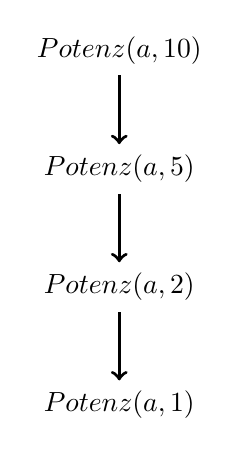
\begin{tikzpicture}[line width=1.2,scale=1.5]
			\node (10) at (0,0) {$\cc{Potenz}(a,10)$};
			\node(5) at (0,-1) {$\cc{Potenz}(a,5)$};
			\node(2) at (0,-2) {$\cc{Potenz}(a,2)$};
			\node(1) at (0,-3) {$\cc{Potenz}(a,1)$};
			\draw[<-]  (1) edge  (2)  (2) edge  (5) (5) edge (10);
		\end{tikzpicture}
	\end{center} 
	Rekursionsbäume mit Verzweigungen erhält man, wenn während der Ausführung einer rekursiven Prozedur mehr als ein rekursiver Aufruf stattfindet. 
\end{bsp} 

\begin{bem}
	Auf der praktischen Seite erfolgt die Umsetzung der Aufrufe von Prozeduren und, insbesondere rekursiven Prozeduren, in Betriebssystemen und Programmiersprachen mit Hilfe des sogenannten Programmstacks. Bei jedem Aufruf wird (intern, auf der Ebene der Maschinensprache) die Stelle im Programm notiert, zu der man nach der Ausführung  der Prozedur zurückkehren soll. Außerdem werden durch einen Aufruf potenziell neue Variablen eingeführt (lokale Variablen der Prozedur, Eingabeparameter). All diese Daten werden auf dem sogenannten \textbf{Aufrufstapel} (engl. call stack, procedure stack) aufgehoben. Die Größe des Aufrufstapels ist standardmäßig ziemlich eingeschränkt, sodass es bei der Ausführung von rekursiven Prozeduren mit einer großen Rekursionstiefe zu einem Überlauf des Aufrufstapels kommen kann. 
	
	In höheren Programmiersprachen, bei denen die Rekursion nicht unbedingt direkt durch den Aufrufstapel umgesetzt wird, wird oft trotzdem das Maximum der Rekursionstiefe festgelegt. 	Hier ein Beispiel eines Python-Codes, der diese Problematik illustriert: 
	\lstinputlisting{Code/dive.py}
	
	Auf meinem Computer führt der Aufruf von dive auf der Eingabe $0$ zu einem Stacküberlauf in der Rekursionstiefe $995$. Die maximale Rekursionstiefe kann oft manuell erhöht werden, und es gibt auch Sprachen, die in gewissen Situationen die rekursiven Prozeduren in nicht-rekursiven Maschinencode übersetzen können. Generell gilt aber: wenn man eine rekursive Prozedur mit einer hohen Rekursionstiefe hat, sollte man sich Gedanken darüber machen, wie man diese Prozedur nicht-rekursiv umsetzen könnte. Sehr oft kann man dabei seinen eigenen Stapel anlegen. 
\end{bem} 

\begin{bsp}[Türme von Hanoi] 
	Gegeben sind drei Stäbe: Startstab, Hilfsstab und Zielstab. Auf dem Startstab sind $n$ Scheiben der Größen $1$ bis $n$ aufgestapelt, so dass die Scheiben von oben nach unten betrachtet nach der Größe steigend sortiert sind. Die Rechenaufgabe besteht darin, eine Folge von Schritten zu bestimmen, mit denen man einzeln alle $n$ Scheiben vom Startstab auf den Zielstab derart versetzt, dass in jedem Schritt die Scheiben von jedem der drei Stäbe sortiert sind (von oben nach unten betrachtet aufsteigend nach der Größe). 
	
	Eine rekursive Lösung dieser Aufgabe sieht so aus: das Ziel ist $n$ Scheiben vom Start $s$ nach Ziel $z$ mit Hilfe von $h$ als Hilfsstab zu versetzen. Wir versetzen die $n-1$ Scheiben vom Start- auf den Hilfsstab, indem wir den Zielstab als Hilfsstab benutzen. Danach wird die größte Scheibe verfügbar: sie kann auf den Zielstab versetzt werden. Danach ist der Startstab frei und kann bei der Versetzung der $n-1$ Scheiben vom Hilfs- auf den Zielstab als Hilfsstab benutzt werden. 
	
	\begin{algorithm}[H]
	\caption{$\cc{Hanoi-Schritte}(n,s,h,z)$}
	\begin{algorithmic}
		\IF{$n=1$ \COMMENT{Terminierungsbedingung} } 
		\PRINT von $s$ nach $z$ 
		\ELSE
		\STATE $\cc{Hanoi-Schritte}(n-1,s,z,h)$ \COMMENT{alle bis auf die größte Scheibe auf $h$}
		\STATE \COMMENT{Wir verschieben die oberste Scheibe endgültig:} 
		\PRINT von $s$ nach $z$ 
		\STATE  $\cc{Hanoi-Schritte}(n-1,h,s,z)$ \COMMENT{die restlichen $n-1$ Scheiben auf $z$} 
		\ENDIF 
	\end{algorithmic}
\end{algorithm}
	Der Rekursionsbaum für $n=3$ ist wie folgt: 
\begin{center} 
	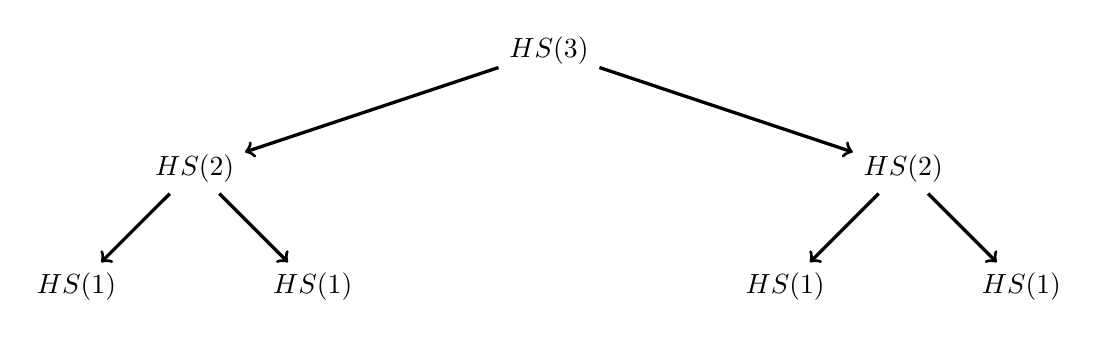
\begin{tikzpicture}[line width=1.2,scale=1.5]
		\node (root) at (0,0) {$\cc{HS}(3)$};
		\node (L) at (-3,-1) {$\cc{HS}(2)$};
		\node (R) at (3,-1) {$\cc{HS}(2)$};
		\node (LL) at (-4,-2)  {$\cc{HS}(1)$};
		\node (LR) at (-2,-2)  {$\cc{HS}(1)$};
		\node (RL) at (2,-2)  {$\cc{HS}(1)$};
		\node (RR) at (4,-2)  {$\cc{HS}(1)$};
		\draw[->]  (root) edge  (L) (root) edge (R) (L) edge (LR) (L) edge (LL) (R) edge (RR) (R) edge (RL);
	\end{tikzpicture}
\end{center} 

	Hierbei steht $\cc{HS}(k)$ für $\cc{Hanoi-Schritte}(k, s,h,z)$ mit irgendeiner Wahl von $s,h,z$. 
	
	Hier Umsetzung in Python mit der Verwendung von Iteratoren: 
\lstinputlisting{Code/hanoi.py}

Eine Demo-Datei für $4$ Türme:
	\begin{center}
	\small{ 
	\url{https://de.wikipedia.org/wiki/T%C3%BCrme_von_Hanoi#/media/Datei:Tower_of_Hanoi_4.gif} } 
	\end{center}

\end{bsp} 

\section{Algorithmen, Rechenprobleme und Komplexität}

\subsection{Random Access Machine}
\label{sect:RAM}

\begin{bem} 
Die \textbf{Random Access Machine} (kurz \textbf{RAM}), oder auf deutsch, \textbf{Maschine mit wahlfreiem Zugriff}, wird unsere \underline{Idealisierung} bzw. mathematische Abstraktion des realen Rechners sein. Alle Analysen und Entwürfe von Algorithmen in diesem Kurs werden im Rahmen der RAM durchgeführt. 

Wir nehmen an, dass die Zellen unserer Maschine ganze Zahlen beliebiger Größe speichern können (d.h., die Bit-Größe der Speicherzellen ist unendlich). Die Speichergröße (d.h., die Anzahl der Speicherzellen) ist ebenfalls unbeschränkt (d.h., unendlich). Wir können des Weiteren alle anderen Datentypen auf der Basis der ganzen Zahlen umsetzen. 

Die Random Access Machine kann auch rein formal eingeführt werden. Wir betrachten hier (zunächst) allerdings eine etwas informelle Beschreibung, in der wir festlegen welche Datentypen, Operationen und Kontrollstrukturen für uns elementar sind. 

Als \textbf{Grundoperationen} für die RAM erlauben wir:
%
\begin{itemize}
	\item Zuweisung (für ganzzahlige Datentypen)
	\item Addition von ganzzahligen Variablen
	\item Multiplikation einer ganzzahligen Variablen mit einer Konstanten
	\item Ganzzahlige Division einer ganzzahligen Variablen durch eine Konstante
	\item Zugriff zu Speicherzellen über einen Index
	\item Vergleichsoperationen $<$, $\le$, $=$, $\ge$, $>$ für ganze Zahlen
	\item Kontrollstrukturen if-then-else, while, for 
\end{itemize}

Eine genauere Beschreibung einer RAM findet man bei \cite[Sect.~1.3]{Lov20}.
\end{bem} 

%Unsere Algorithmen werden als Pseudocode formuliert und ihre Analyse wird im Rahmen dieses Modells durchgeführt. Für Pseudocode legen wir fest, dass standardmäßig in Prozeduren alle einfachen Datentypen durch Kopie und alle komplexen Datentypen (Arrays usw.) durch Referenz übergeben werden. 

\begin{bem} 
Wir lassen die Multiplikation von zwei ganzzahligen Variablen in unserem Modell nicht als Grundoperation zu. Denn, wenn das eine Grundoperation wäre, so hätte der folgende Algorithmus die Laufzeit $O(n)$: 

\begin{center}
	\begin{algorithmic}
		\STATE $x:=2$
		\FOR{$i=1,\ldots,n$} 
		\STATE $x:=x^2$
		\ENDFOR
	\end{algorithmic}
\end{center}

Dieser Algorithmus würde also $2^{2^n}$ in der Zeit $O(n)$ berechnen. Die Zahl $2^{2^n}$ hat allerdings $2^n+1$ Binärstellen. Wir würden also eine Zahl exponentieller Bit-Größe in linearer Zeit berechnen, was wir als unrealistisch ansehen. 
\end{bem}


\subsection{Rechenprobleme und Sprachen}
\label{sect:rechenprobleme}

\begin{defn}
	Wir fixieren die \textbf{Standard-Kodierungen} durch Bit-Strings für Mengen $\Z, \Q$ sowie $\Z^n$ und $\Q^n$ mit $n \in \N$ wie folgt: 
	\begin{itemize}
		\item Für $z \in \Z$ ist die Standard-Kodierung die Darstellung von $z$ im Binärsystem. Diese Kodierung hat die Größe $\Theta(\log_2 (|z|+1))$. 
		\item Jedes $q \in \Q$ kann eindeutig als $q = a/b$ mit $a \in \Z$ und $b \in \N$ fixiert werden. Danach wird das Paar $(a,b) \in \Z \times \N$ mit der Verwendung der Standardkodierungen von $a$ und $b$ kodiert (vgl. dazu den Beweis der Proposition~\ref{kod:paare} über das Kodieren von Paaren). 
		\item $\Z^n$ und $\Q^n$ wird in Anlehnung an die oben festgelegten Standardkodierungen von $\Z$ und $\Q$ kodiert (vgl.~Korollar~\ref{kod:tupel}). 
	\end{itemize} 
	Für ein Element $x$ aus einer dieser Mengen ($\Z,\Q, \Z^n$ oder $\Q^n$) bezeichnen wir als $\enc{x} \in \{0,1\}^\ast$ die Standardkodierung von $x$ und als $\encl{x}$ die Länge dieser Kodierung. 
\end{defn} 

\begin{defn}
	Ein \textbf{Rechenproblem} ist eine binäre Relation auf der Menge der Bit-Strings $\{0,1\}^\ast$. Mit anderen Worten ist ein Rechenproblem eine Menge 
	\[
	\Pi \subseteq \{0,1\}^\ast \times \{0,1\}^\ast.
	\]
	Die Bedeutung von $(x,y) \in \Pi$ ist dabei: $y$ ist eine mögliche Rückgabe für die Eingabe $x$. Somit ist ein Rechenproblem eine \textbf{Eingabe-Rückgabe-Relation}. Ein Rechenproblem~$\Pi$ \textbf{algorithmisch zu lösen} heißt, einen Algorithmus zu finden, der für jede Eingabe $x$ entscheidet, ob ein $y$ mit $(x,y) \in \Pi$ existiert und ggf. ein solches $y$ berechnet. 
\end{defn} 

\begin{bem}
	Die Berechnung einer Funktion $f : \{0,1\}^\ast \to \{0,1\}^\ast$ ist ein Spezialfall eines Rechenproblems, bei dem es für jede Eingabe $x$ eine eindeutige Rückgabe $f(x)$ gibt. 
\end{bem} 

\begin{defn}
	Eine Teilmenge $L \subseteq \{0,1\}^\ast$ nennt man \textbf{Sprache}. Eine Sprache \textbf{algorithmisch zu entscheiden} heißt, einen Algorithmus zu finden, der für jedes $x \in \{0,1\}^\ast$ entscheidet, ob $x$ zu $L$ gehört oder nicht. Die Entscheidung der Sprache $L$ kann als die Berechnung der Funktion $f : \{0,1\}^\ast \to \{0,1\}$ mit 
	\[
	f(x) := \begin{cases}
		1 & \text{für} \ x \in L
		\\ 0 & \text{für} \ x \not\in L
	\end{cases} 
	\]
	formuliert werden. Die Rechenprobleme, die durch eine Sprache definiert werden, nennt man \textbf{Entscheidungsprobleme}. Es handelt sich dabei um Probleme, bei denen man nur zwei mögliche Rückgabewerte hat (ja/nein bzw. wahr/falsch bzw. 1/0). 
\end{defn}

\begin{bem}
	Die vorigen Definitionen werden wir auch mit anderen Mengen an der Stelle von $\{0,1\}^\ast$ benutzen, unter der Voraussetzung, dass für diese Mengen eine Kodierung mit Bit-Strings festgelegt ist:
	\begin{itemize}
		\item Ein Rechenproblem ist eine Eingabe-Rückgabe-Relation $\Pi \subseteq  X \times Y$ für die Menge $X$ aller möglichen Eingaben (mit einer festgelegten Kodierung der Eingabe) und die Menge~$Y$ aller möglichen Rückgaben (mit einer festgelegten Kodierung der Rückgabe). 
		\item Analog kann das Problem der algorithmischen Berechnung einer Abbildung $f : X \to Y$ beschrieben werden, sobald Kodierungen für $X$ und $Y$ festgelegt sind. 
		\item Entscheidungsprobleme entsprechen der algorithmischen Berechnung von Prädikaten der Form $P : X \to \{\false,\true\}$. 
	\end{itemize} 
\end{bem} 

\begin{bsp}\ 
	\begin{itemize} 
		\item Das Problem
		\[
		\setcond{ (a,p) \in \N \times \Z_{\ge 2} }{p \ \text{ist Primfaktor von} \ a} \subseteq \N \times \Z_{\ge 2}
		\]
		kann mit Worten folgendermaßen formuliert werden: entscheide, für ein gegebenes $a \in \N$, ob $a$ einen Primfaktor $p \in \Z_{\ge 2}$ besitzt und berechne ggf. einen solchen Faktor. 
		\item Die Berechnung von $f : \Z \times \N_0 \to \N$ mit $f(a,k):= a^k$ kann mit Worten so formuliert werden: für gegebene $a \in \Z,k \in \N_0$ berechne die $k$-te Potenz von $a$. 
		\item Das algorithmische  Problem zur Sprache der (Bit-Kodierungen von) Primzahlen ist zu entscheiden, ob die Eingabe (die Bit-Kodierung einer) Primzahl ist. Mit Worten: entscheide, ob eine gegebene Zahl $z \in \N$ eine Primzahl ist. 
	\end{itemize} 
\end{bsp} 

\subsection{Entscheidbarkeit}

\begin{defn}
	Eine Sprache $L \subseteq \{0,1\}^\ast$ heißt \textbf{entscheidbar}, wenn ein Algorithmus existiert, der die Sprache~$L$ entscheidet. 
\end{defn} 

\begin{lem} \label{lem:X:2^X}
	Sei $X$ eine Menge. Dann gibt es keine surjektive Abbildung $F : X \to 2^X$. 
\end{lem}
\begin{proof}
Sei $F : X \to 2^X$ eine Abbildung.
	Man betrachte die Menge $Y := \setcond{x \in X}{x \not\in F(x)}$. Wir zeigen durch ein Widerspruchsargument, dass kein $a \in X$ mit $F(a) =Y$ existiert. Angenommen, es gäbe ein solches $a$. 
	
	Hat man $a \in Y$, so ist $a \in F(a)$, weil $Y=F(a)$ ist. Aber andererseits besteht $Y$ aus allen $x \in X$, für die $x \not\in F(x)$ gilt, sodass wegen $a \in Y$ auch gleichzeitig $a \not\in F(a)$ gilt. Widerspruch. 
	
	Hat man $a \not\in Y$, so ist $a \not\in F(a)$, weil $Y=F(a)$ ist. Aber andererseits besteht $Y$ genau aus den $x \in X$ mit $x \not\in F(x)$. Wegen $a \not\in Y$ gilt damit $a \in F(a)$. Widerspruch. 
\end{proof} 

\begin{thm}
	Es existieren Sprachen, die nicht entscheidbar sind. 
\end{thm} 
\begin{proof} 
		Ein Algorithmus ist durch seinen \glqq Quellcode\grqq\ darstellbar. Denn ein jeder Algorithmus ist eine Auflistung von Grundbefehlen, die man alle mit Hilfe von Strings über einem endlichen Alphabet darstellen kann. Somit kann  man jeden Algorithmus als ein String über einem endlichen Alphabet kodieren. Wir identifizieren also die Algorithmen mit Elementen von $\{0,1\}^\ast$. Die Menge aller Sprachen über dem Alphabet $\{0,1\}^\ast$ ist die Menge $2^{\{0,1\}^\ast}$. Wäre jede Sprache entscheidbar, so könnte man für jede Sprache $L \in 2^{\{0,1\}^\ast}$ einen Algorithmus (genauer: Quellcode eines Algorithmus) $A_L \in \{0,1\}^\ast$ fixieren, der die Sprache $L$ entscheidet. Wir können also eine Abbildung $F : \{0,1\}^\ast \to 2^{\{0,1\}^\ast}$ so fixieren, dass $F(A_L) = L$ für alle $L \in 2^{\{0,1\}^\ast}$ gilt. Die Abbildung $F$ ist surjektiv. Die Existenz der Abbildung $F$ widerspricht aber der Behauptung von Lemma~\ref{lem:X:2^X}.
\end{proof} 

\subsection{Komplexität im Hinblick auf die Laufzeit} 

\begin{defn} 
	Sei $A$ ein Algorithmus im Rahmen eines Rechenmodells, dessen Schritte als Grundoperationen im gegebenen Rechenmodell beschrieben sind. 

Die \textbf{Laufzeit} $L(A,x)$ von~$A$ auf der Eingabeinstanz $x$ ist die Anzahl der Schritte des Algorithmus $A$ auf der Eingabe $x$ bis zur Terminierung. 

Für eine Menge $X$ von Eingabe-Instanzen, heißt $\max_{x \in A} L(A,x)$ die \textbf{Worst-Case-Laufzeit} von $A$ auf $X$. 

Die \textbf{Laufzeitfunktion} $L_A : \N \to \N$ von~$A$ beschreibt die Worst-Case-Laufzeit in Abhängigkeit von einer oberen Schranke an die Länge der Eingabe: 
\[
L_A(n) := \max \setcond{  L(A,x) }{x \ \text{Eingabe für} \ A  \ \text{mit} \ \encl{x} \le n}.
\]
\end{defn} 

\begin{defn}
	Eine Funktion $p : \R \to \R$ heißt \textbf{Polynomfunktion} vom Grad $d \in \N_0$, falls~$p$ die Form \[
		p(t)= c_0 + c_1 t + c_2 t^2 + \ldots + c_d t^d
	\]
	hat, mit $c_0,\ldots,c_d \in \R$ und $c_d \ne 0$. 
\end{defn} 

\begin{defn} 
Wir nennen einen Algorithmus~$A$ \textbf{polynomial} oder \textbf{Polynomialzeit-Algorithmus} (bezüglich des zugrundeliegenden Rechenmodells und Kodierungsschemas für die Eingabe), falls eine Polynomfunktion~$p$ existiert, so dass $L_A(n) \leq p(n)$ für alle $n \in \N_0$ gilt.
\end{defn} 

\begin{bem}
	Ein Polynomialzeit-Algorithmus $A$ ist ein Algorithmus, deren Laufzeitfunktion die Ordnung $O(n^d)$, für ein $d \in \N_0$, hat. 
\end{bem} 

\begin{bem}
	In der Theorie nennt man Polynomialzeit-Algorithmen oft auch \textbf{effiziente} Algorithmen. Welche Algorithmen aus der praktischen Sicht effizient sind, lässt sich schwer formal beschreiben.
\end{bem} 

\begin{defn}
	Für $T: \N_0 \to \N$ heißt ein Rechenproblem \textbf{in der Zeit $T(n)$} berechenbar, wenn ein Algorithmus $A$ existiert, der das Problem löst und dessen Laufzeit-Funktion die Bedingung $L_A(n) \le T(n)$ für alle $n \in \N_0$ erfüllt. Im Fall von Sprachen sagt man \glqq in der Zeit $T(n)$ entscheidbar\grqq. 
	
	Ein Rechenproblem heißt \textbf{Polynomialzeit-berechenbar}, wenn es einen Po\-ly\-no\-mi\-al\-zeit-Algorithmus gibt, der das Rechenproblem löst. 
	
	Ein Entscheidungsproblem bzw. eine Sprache heißt \textbf{Polynomialzeit-\-ent\-scheid\-bar}, wenn ein Polynomialzeit-Algorithmus existiert, der das Problem bzw. die Sprache entscheidet. 
\end{defn} 

\begin{bem}
	Die Berechenbarkeit in der Zeit $T(n)$ bezieht sich auf ein zugrundeliegendes Rechenmodell. Das ist die RAM in unserem Fall, es gibt aber auch andere Rechenmodelle (z.B. Modelle, die nur einen sequentiellen Zugriff zu den Speicherzellen ermöglichen). 
\end{bem} 

\begin{defn}
	Die Menge aller Polynomialzeit-entscheidbaren Sprachen $L \subseteq \{0,1\}^\ast$ wird die \textbf{Komplexitätsklasse} $\operatorname{P}$ genannt. Als formaler Ausdruck: 
	\[
			\DP := \setcond{L \subseteq \{0,1\}^\ast }{L \ \text{Polynomialzeit-entscheidbar} } .
	\]
\end{defn} 

\begin{defn}
	Als $\EXP$ bezeichnet man die Menge aller Sprachen $L$, für die ein Polynom $p$ existiert, sodass $L$  in der Zeit $2^{p(n)}$ entscheidbar ist. 
\end{defn} 

\begin{bem}
	Es gilt $\DP\subseteq \EXP$ und man kann sogar zeigen, dass diese Inklusion strikt ist. 
\end{bem} 

\subsection{Übersetzungen und Vergleiche von Sprachen}

\begin{defn}
	Seien $L$ und $M$ Sprachen über dem Alphabet $\{0,1\}$. Man nennt $L$ \textbf{Polynomialzeit-Karp-reduzierbar} zu $M$ (Bezeichnung: $L \le_{\DP} M$) wenn eine Polynomialzeit-Berechenbare Abbildung $f : \{0,1\}^\ast \to \{0,1\}^\ast$ existiert mit 
	\[
		L = \setcond{x \in \{0,1\}^\ast}{ f(x) \in M}.
	\]  
	Man nennt dabei $f$ bzw. den Algorithmus zur Berechnung von $f$ die \textbf{Polynomialzeit-Karp-Reduktion} von $L$ zu $M$. 
	
	Wir nennen $L$ und $M$ Polynomialzeit-Karp-äquivalent, wenn $L \le_{\DP} M$ und $M \le_{\DP} L$ erfüllt ist. In diesem Fall benutzen wir die Bezeichnung $L  =_{\DP} M.$ 
\end{defn} 

\begin{prop}
	Ist $M \in \DP$ und $L \le_{\DP} M$, so ist auch $L \in \DP$. 
\end{prop} 

\begin{bem}
	Die kontrapositive Form der vorigen Aussage ist auch nützlich. 
\end{bem}

\begin{prop}
	Ist $L \not\in \DP$ und $L \le_{\DP} M$, so ist auch $M \not\in DP$. 
\end{prop} 

IM AUFBAU 

